\documentclass[a4paper,12pt]{article}

\usepackage{graphicx}
\usepackage{amsmath}
\usepackage{hyperref}
\usepackage{caption}
\usepackage{subcaption}
\usepackage{circuitikz}

\title{\textbf{Lab Report: Experiment 5}}
\author{EE1200 - IIT Hyderabad}
\date{\today}

\begin{document}
\maketitle

\begin{center}
    \textbf{Experiment:}Op-Amp Applications
\end{center}
\vspace{30pt}

\begin{figure}[h!]
    \centering
    
\includegraphics[width = 100pt]{.logo/logo.png}\\
\end{figure}

\begin{center}
    Bachelor of Technology\\
    \vspace{10pt}
    Department of Electrical Engineering\\
\end{center}
\newpage

\section*{Objective}
The objective of this experiment is to analyze and implement three operational amplifier applications:
\begin{enumerate}
    \item Custom Weighted Summing and Difference Amplifier
    \item Op-Amp Integrator
    \item Precision Rectifier (Super Diode)
\end{enumerate}

\section*{Components Required}
\begin{itemize}
	\item Operational Amplifier (LM 358)
    \item Resistors (selected for proper weighting)
    \item DC Power Supply
    \item Function Generator
    \item Oscilloscope
\end{itemize}

\section*{Theory and Circuit Design}
\subsection*{Custom Weighted Summing and Difference Amplifier}
This circuit implements the mathematical functions:
\begin{align}
    V_{out} &= 2V_1 + V_2 - V_3 \\
    V_{out} &= 2V_1 - V_3
\end{align}
An inverting summing amplifier is used with appropriately chosen resistor values to achieve the desired coefficients.
The output of an inverting summing amplifier is given by
\begin{align}
	V_{out} = -(\frac{R_f}{R_1} V_1 + \frac{R_f}{R_2} V_2)
\end{align}
By taking $R_f = 2R, R_1 = R$ and $R_2 = 2R$,
\begin{align}
	V_{out} = -(2V_1 + V_2)
\end{align}
Now by taking the output of this op amp and summing this output with another input voltage $V_3$ will give us the required output voltage. The output of the second op amp will be,
\begin{align}
	V_{out} = -(\frac{R_f}{R_1} (-2V_1 - V_2) + \frac{R_f}{R_2} V_3)
\end{align}
Taking $R_f = R_1 = R_2 = R$,
\begin{align}
	V_{out} = (2V_1 + V_2 - V_3)
\end{align}

\subsection*{Circuit Diagram}

\begin{figure}[!ht]
\centering
\resizebox{1\textwidth}{!}{%
\begin{circuitikz}
\tikzstyle{every node}=[font=\LARGE]
\draw (10.25,14.75) node[op amp,scale=1] (opamp2) {};
\draw (opamp2.+) to[short] (8.75,14.25);
\draw  (opamp2.-) to[short] (8.75,15.25);
\draw (11.45,14.75) to[short](11.75,14.75);
\draw (8.25,14.25) to (8.25,13.25) node[ground]{};
\draw (8.25,15.25) to[short] (8.25,16.75);
\draw (8.25,16.75) to[R] (6.5,16.75);
\draw (15.5,14.25) node[op amp,scale=1] (opamp2) {};
\draw (opamp2.+) to[short] (14,13.75);
\draw  (opamp2.-) to[short] (14,14.75);
\draw (16.7,14.25) to[short](17,14.25);
\draw (14,13.75) to (14,12.75) node[ground]{};
\draw (8.25,15.75) to[R] (6.5,15.75);
\node at (6.5,16.75) [circ] {};
\node at (6.5,15.75) [circ] {};
\node at (17,14.25) [circ] {};
\node [font=\normalsize] at (6,16.75) {$V_1$};
\node [font=\normalsize] at (6,15.75) {$V_2$};
\node [font=\normalsize] at (12.5,15.25) {};
\node [font=\normalsize] at (18.25,14.25) {$2V_1 + V_2 - V_3$};
\draw (8.25,15.25) to[short] (8.75,15.25);
\draw (8.25,14.25) to[short] (9,14.25);
\draw (8.75,15.25) to[short] (8.75,16.5);
\draw (11,16.25) to[short] (11,14.75);
\draw (8.75,16.5) to[R] (11,16.5);
\draw (11,16.5) to[short] (11,16);
\draw (14.25,14.75) to[short] (14.25,16);
\draw (16.5,16) to[short] (16.5,14.25);
\draw (14.25,16) to[R] (16.5,16);
\draw (13,14.75) to[R] (14,14.75);
\draw (9.5,11.5) to[short] (12.5,11.5);
\draw (12.5,11.5) to[short] (12.5,14);
\draw (6.5,11.5) to[R] (8.25,11.5);
\draw (14.25,14.75) to[short] (14.25,14);
\draw (14.25,14) to[short] (13.75,14);
\node at (6.5,11.5) [circ] {};
\node [font=\normalsize] at (6,11.5) {$V_3$};
\node [font=\normalsize] at (10,17) {2R};
\node [font=\normalsize] at (15.25,16.5) {R};
\node [font=\normalsize] at (13.5,15.25) {R};
\node [font=\normalsize] at (7.25,11) {R};
\node [font=\normalsize] at (7.25,17.25) {R};
\node [font=\normalsize] at (7.25,15.25) {2R};
\node at (11,14.75) [circ] {};
\node [font=\normalsize] at (11.5,14.25) {$-2V_1 - V_2$};
\draw (11.75,14.75) to[short] (13,14.75);
\draw (8.25,11.5) to[short] (10.25,11.5);
	\node [font=\normalsize] at (7.5,10.75) {};
\draw (12.5,14) to[short] (14,14);
\end{circuitikz}
}%
\label{fig:my_label}
\end{figure}

For the second part, to produce output voltage of $2V_1 - V_3$, make $V_2 = 0$, i.e., ground the terminal connecting $V_2$.

\subsection*{Circuit Diagram}
\begin{figure}[!ht]
\centering
\resizebox{1\textwidth}{!}{%
\begin{circuitikz}
\tikzstyle{every node}=[font=\normalsize]
\draw (10.25,14.75) node[op amp,scale=1] (opamp2) {};
\draw (opamp2.+) to[short] (8.75,14.25);
\draw  (opamp2.-) to[short] (8.75,15.25);
\draw (11.45,14.75) to[short](11.75,14.75);
\draw (8.25,14.25) to (8.25,13.25) node[ground]{};
\draw (8.25,15.25) to[short] (8.25,16.75);
\draw (8.25,16.75) to[R] (6.5,16.75);
\draw (15.5,14.25) node[op amp,scale=1] (opamp2) {};
\draw (opamp2.+) to[short] (14,13.75);
\draw  (opamp2.-) to[short] (14,14.75);
\draw (16.7,14.25) to[short](17,14.25);
\draw (14,13.75) to (14,12.75) node[ground]{};
\draw (8.25,15.75) to[R] (6.5,15.75);
\node at (6.5,16.75) [circ] {};
\node at (6.5,15.75) [circ] {};
\node at (17,14.25) [circ] {};
\node [font=\normalsize] at (6,16.75) {$V_1$};
\node [font=\normalsize] at (5.75,15.75) {$V_2 = 0$};
\node [font=\normalsize] at (12.5,15.25) {};
\node [font=\normalsize] at (18.25,14.25) {$2V_1 - V_3$};
\draw (8.25,15.25) to[short] (8.75,15.25);
\draw (8.25,14.25) to[short] (9,14.25);
\draw (8.75,15.25) to[short] (8.75,16.5);
\draw (11,16.25) to[short] (11,14.75);
\draw (8.75,16.5) to[R] (11,16.5);
\draw (11,16.5) to[short] (11,16);
\draw (14.25,14.75) to[short] (14.25,16);
\draw (16.5,16) to[short] (16.5,14.25);
\draw (14.25,16) to[R] (16.5,16);
\draw (13,14.75) to[R] (14,14.75);
\draw (9.5,11.5) to[short] (12.5,11.5);
\draw (12.5,11.5) to[short] (12.5,14);
\draw (6.5,11.5) to[R] (8.25,11.5);
\draw (14.25,14.75) to[short] (14.25,14);
\draw (14.25,14) to[short] (13.75,14);
\node at (6.5,11.5) [circ] {};
\node [font=\normalsize] at (6,11.5) {$V_3$};
\node [font=\normalsize] at (10,17) {2R};
\node [font=\normalsize] at (15.25,16.5) {R};
\node [font=\normalsize] at (13.5,15.25) {R};
\node [font=\normalsize] at (7.25,11) {R};
\node [font=\normalsize] at (7.25,17.25) {R};
\node [font=\normalsize] at (7.25,15.25) {2R};
\node at (11,14.75) [circ] {};
\node [font=\normalsize] at (11.5,14.25) {$-2V_1 - V_2$};
\draw (11.75,14.75) to[short] (13,14.75);
\draw (8.25,11.5) to[short] (10.25,11.5);
\node [font=\normalsize] at (7.5,10.75) {};
\draw (12.5,14) to[short] (14,14);
\draw (6.5,15.75) to (6.5,15) node[ground]{};
\end{circuitikz}
}%
\label{fig:my_label}
\end{figure}


\pagebreak
\subsection*{Op-Amp Integrator}
This circuit performs mathematical integration:
\begin{equation}
    V_{out} = - \frac{1}{RC} \int V_{in} dt
\end{equation}
In the below circuit, on applying nodal analysis at point $A$, 
\begin{align}
	\frac{V_a - V_{in}}{R} + I_C &= 0\\
	\frac{V_a - V_{in}}{R} + C\frac{dV_C}{dt} &= 0
\end{align}
In case of an ideal op amp, $V_A = 0$,
\begin{align}
	\frac{V_{in}}{R} &= C\frac{dv}{dt}\\
	\int{dv} &= \frac{1}{RC}\int{V_{in}} dt\\
	0 - V_{out} &= \frac{1}{RC}\int{V_{in}} dt\\
	V_{out} &= -\frac{1}{RC}\int{V_{in}} dt
\end{align}

\pagebreak
\subsection*{Circuit Diagram}

\begin{figure}[!ht]
\centering
\resizebox{0.5\textwidth}{!}{%
\begin{circuitikz}
\tikzstyle{every node}=[font=\normalsize]
\draw (14.25,14.25) node[op amp,scale=1] (opamp2) {};
\draw (opamp2.+) to[short] (12.75,13.75);
\draw  (opamp2.-) to[short] (12.75,14.75);
\draw (15.45,14.25) to[short](15.75,14.25);
\draw (10.5,14.75) to[R] (12.75,14.75);
\draw (12.75,13.75) to (12.75,12.5) node[ground]{};
\draw (12.75,14.75) to[short] (12.75,16.5);
\draw (12.75,16.5) to[C] (15.5,16.5);
\draw (15.5,16.5) to[short] (15.5,14.25);
\draw (15.75,14.25) to[short] (16.25,14.25);
\node at (10.5,14.75) [circ] {};
\node at (16.25,14.25) [circ] {};
\node [font=\normalsize] at (10,14.75) {$V_{in}$};
\node [font=\normalsize] at (14.25,17.25) {$C$};
\node [font=\normalsize] at (16.75,14.25) {$V_{out}$};
\node [font=\normalsize] at (11.5,15.25) {$R$};
\node [font=\normalsize] at (12.75,14.5) {$A$};
\node at (12.75,14.75) [circ] {};
\draw [->, >=Stealth] (12.75,15.25) -- (12.75,15.75);
\node [font=\normalsize] at (12.25,15.75) {$I_C$};
\end{circuitikz}
}%
\label{fig:my_label}
\end{figure}

\section*{Precision Rectifier}
Here, the aim is to use the op amp to control a diode for full-wave rectifier and a half-wave rectifier.
The reason why we use the op amp is because the diode has a threshold voltage of $0.7V$. To reduce that voltage to $0V$, we use the op amp. Depending on the amount of load resistance given to the op amp, a full or a half wave rectifier can be achieved.

\subsection*{Circuit Diagram}

\subsubsection*{Half wave rectifier}
\pagebreak
\begin{figure}[!ht]
\centering
\resizebox{0.5\textwidth}{!}{%
\begin{circuitikz}
\tikzstyle{every node}=[font=\normalsize]
\draw[domain=5:12.75,samples=100,smooth] plot (\x,{1.3*sin(5*\x r -5 r ) + 17.5});
\draw[domain=5.4:6.03,samples=100,smooth] plot (\x,-{1.3*sin(5*\x r -5 r ) +13.75});
\draw[domain=6.65:7.28,samples=100,smooth] plot (\x,-{1.3*sin(5*\x r -5 r ) +13.75});
\draw[domain=7.91:8.54,samples=100,smooth] plot (\x,-{1.3*sin(5*\x r -5 r ) +13.75});
\draw[domain=9.17:9.8,samples=100,smooth] plot (\x,-{1.3*sin(5*\x r -5 r ) +13.75});
\draw[domain=10.43:11.06,samples=100,smooth] plot (\x,-{1.3*sin(5*\x r -5 r ) +13.75});
\draw[domain=11.68:12.31,samples=100,smooth] plot (\x,-{1.3*sin(5*\x r -5 r ) +13.75});
\draw [->, >=Stealth] (5,17.5) -- (13.5,17.5);
\draw [->, >=Stealth] (5,16) -- (5,19.25);
\draw [->, >=Stealth] (5,13.75) -- (13.5,13.75);
\draw [->, >=Stealth] (5,13.25) -- (5,15.5);
\node [font=\normalsize] at (5,19.5) {$V_{in}$};
\node [font=\normalsize] at (5,15.75) {$V_{out}$};
\end{circuitikz}
}%
\label{fig:my_label}
\end{figure}
\textbf{Negative Half Cycle:}
The upper diode is in reverse-bias condition while the lower diode is in forward-bias condition. This will lead to $V_{out} = -\left(\frac{R_2}{R_1}\right)V_{in}$. Here, $R_2 = R_1$, so $V_{out} = -V_{in}$. \newline


\begin{figure}[!ht]
\centering
\resizebox{0.5\textwidth}{!}{%
\begin{circuitikz}
\tikzstyle{every node}=[font=\normalsize]
\draw (14,14) node[op amp,scale=1] (opamp2) {};
\draw (opamp2.+) to[short] (12.5,13.5);
\draw  (opamp2.-) to[short] (12.5,14.5);
\draw (15.2,14) to[short](15.5,14);
\draw (12.5,14.5) to[R] (10.25,14.5);
\draw (12.5,13.5) to (12.5,12.25) node[ground]{};
\draw (12.5,14.5) to[short] (12.5,16.25);
%\draw (12.5,16.25) to[D] (15.25,16.25);
\draw(12.5, 16.25) to (13.25, 16.25);
\draw (14.25, 16.25) to (15.25, 16.25);
\draw (15.25,16.25) to[short] (15.25,14);
\draw (15.5,14) to[D] (17.5,14);
\draw (12.5,16.25) to[short] (12.5,17.25);
\draw (12.5,17.25) to[R] (17.25,17.25);
\draw (17.25,17.25) to[short] (17.25,14);
\draw (17.5,14) to[short] (18,14);
\draw (18,14) to[R] (18,12.25);
\draw (18,12.5) to (18,12.25) node[ground]{};
\node at (10.25,14.5) [circ] {};
\node at (12.5,16.25) [circ] {};
\node at (12.5,14.5) [circ] {};
\node at (15.25,14) [circ] {};
\node at (17.25,14) [circ] {};
\node [font=\normalsize] at (15,17.75) {$R_2$};
\node [font=\normalsize] at (11.25,15) {$R_1$};
\node [font=\normalsize] at (18.75,13) {$R_3$};
\draw (10.25,14.5) to[sinusoidal voltage source, sources/symbol/rotate=auto] (10.25,12.25);
\draw (10.25,12.5) to (10.25,12.25) node[ground]{};
\node [font=\normalsize] at (9.5,13.25) {$V_{in}$};
\node [font=\normalsize] at (17.75,14.25) {$V_{out}$};
\end{circuitikz}
}%
\label{fig:my_label}
\end{figure}
\textbf{Positive Half Cycle:}
The lower diode is in reverse-bias condition, while the upper diode is in forward-bias condition. So there is no path for current to flow, so $V_{out} = V_- = V_+ = 0$
\begin{figure}[!h]
\centering
\resizebox{0.5\textwidth}{!}{%
\begin{circuitikz}
\tikzstyle{every node}=[font=\normalsize]
\draw (14,14) node[op amp,scale=1] (opamp2) {};
\draw (opamp2.+) to[short] (12.5,13.5);
\draw  (opamp2.-) to[short] (12.5,14.5);
\draw (15.2,14) to[short](15.5,14);
\draw (12.5,14.5) to[R] (10.25,14.5);
\draw (12.5,13.5) to (12.5,12.25) node[ground]{};
\draw (12.5,14.5) to[short] (12.5,16.25);
\draw (12.5,16.25) to[D] (15.25,16.25);
%\draw(12.5, 16.25) to (13.25, 16.25);
\draw (14.25, 16.25) to (15.25, 16.25);
\draw (15.25,16.25) to[short] (15.25,14);
%\draw (15.5,14) to[D] (17.5,14);
\draw (15.5, 14) to (15.75, 14);
\draw(16.5, 14) to (17.5, 14);
\draw (12.5,16.25) to[short] (12.5,17.25);
\draw (12.5,17.25) to[R] (17.25,17.25);
\draw (17.25,17.25) to[short] (17.25,14);
\draw (17.5,14) to[short] (18,14);
\draw (18,14) to[R] (18,12.25);
\draw (18,12.5) to (18,12.25) node[ground]{};
\node at (10.25,14.5) [circ] {};
\node at (12.5,16.25) [circ] {};
\node at (12.5,14.5) [circ] {};
\node at (15.25,14) [circ] {};
\node at (17.25,14) [circ] {};
\node [font=\normalsize] at (15,17.75) {$R_2$};
\node [font=\normalsize] at (11.25,15) {$R_1$};
\node [font=\normalsize] at (18.75,13) {$R_3$};
\draw (10.25,14.5) to[sinusoidal voltage source, sources/symbol/rotate=auto] (10.25,12.25);
\draw (10.25,12.5) to (10.25,12.25) node[ground]{};
\node [font=\normalsize] at (9.5,13.25) {$V_{in}$};
\node [font=\normalsize] at (17.75,14.25) {$V_{out}$};
\end{circuitikz}
}%
\label{fig:my_label}
\end{figure}
\newline
\textbf{Circuit Diagram}
\begin{figure}[!h]
\centering
\resizebox{0.5\textwidth}{!}{%
\begin{circuitikz}
\tikzstyle{every node}=[font=\normalsize]
\draw (14,14) node[op amp,scale=1] (opamp2) {};
\draw (opamp2.+) to[short] (12.5,13.5);
\draw  (opamp2.-) to[short] (12.5,14.5);
\draw (15.2,14) to[short](15.5,14);
\draw (12.5,14.5) to[R] (10.25,14.5);
\draw (12.5,13.5) to (12.5,12.25) node[ground]{};
\draw (12.5,14.5) to[short] (12.5,16.25);
\draw (12.5,16.25) to[D] (15.25,16.25);
\draw (15.25,16.25) to[short] (15.25,14);
\draw (15.5,14) to[D] (17.5,14);
\draw (12.5,16.25) to[short] (12.5,17.25);
\draw (12.5,17.25) to[R] (17.25,17.25);
\draw (17.25,17.25) to[short] (17.25,14);
\draw (17.5,14) to[short] (18,14);
\draw (18,14) to[R] (18,12.25);
\draw (18,12.5) to (18,12.25) node[ground]{};
\node at (10.25,14.5) [circ] {};
\node at (12.5,16.25) [circ] {};
\node at (12.5,14.5) [circ] {};
\node at (15.25,14) [circ] {};
\node at (17.25,14) [circ] {};
\node [font=\normalsize] at (15,17.75) {$1 k\Omega$};
\node [font=\normalsize] at (11.25,15) {$1 k\Omega$};
\node [font=\normalsize] at (18.75,13) {$180 \Omega$};
\draw (10.25,14.5) to[sinusoidal voltage source, sources/symbol/rotate=auto] (10.25,12.25);
\draw (10.25,12.5) to (10.25,12.25) node[ground]{};
\node [font=\normalsize] at (9.5,13.25) {$V_{in}$};
\node [font=\normalsize] at (17.75,14.25) {$V_{out}$};
\end{circuitikz}
}%
\label{fig:my_label}
\end{figure}
\pagebreak

\subsubsection*{Full wave rectifier}
\begin{figure}[!ht]
\centering
\resizebox{0.5\textwidth}{!}{%
\begin{circuitikz}
\tikzstyle{every node}=[font=\normalsize]
\draw[domain=5:12.75,samples=100,smooth] plot (\x,{1.3*sin(5*\x r -5 r ) + 17.5});
\draw[domain=5:5.4,samples=100,smooth] plot (\x,{1.3*sin(5*\x r -5 r ) +13.75});
\draw[domain=5.4:6.03,samples=100,smooth] plot (\x,-{1.3*sin(5*\x r -5 r ) +13.75});
\draw[domain=6.03:6.65,samples=100,smooth] plot (\x,{1.3*sin(5*\x r -5 r ) +13.75});
\draw[domain=6.65:7.28,samples=100,smooth] plot (\x,-{1.3*sin(5*\x r -5 r ) +13.75});
\draw[domain=7.28:7.91,samples=100,smooth] plot (\x,{1.3*sin(5*\x r -5 r ) +13.75});
\draw[domain=7.91:8.54,samples=100,smooth] plot (\x,-{1.3*sin(5*\x r -5 r ) +13.75});
\draw[domain=8.54:9.17,samples=100,smooth] plot (\x,{1.3*sin(5*\x r -5 r ) +13.75});
\draw[domain=9.17:9.8,samples=100,smooth] plot (\x,-{1.3*sin(5*\x r -5 r ) +13.75});
\draw[domain=9.8:10.43,samples=100,smooth] plot (\x,{1.3*sin(5*\x r -5 r ) +13.75});
\draw[domain=10.43:11.06,samples=100,smooth] plot (\x,-{1.3*sin(5*\x r -5 r ) +13.75});
\draw[domain=11.06:11.68,samples=100,smooth] plot (\x,{1.3*sin(5*\x r -5 r ) +13.75});
\draw[domain=11.68:12.31,samples=100,smooth] plot (\x,-{1.3*sin(5*\x r -5 r ) +13.75});
\draw [->, >=Stealth] (5,17.5) -- (13.5,17.5);
\draw [->, >=Stealth] (5,16) -- (5,19.25);
\draw [->, >=Stealth] (5,13.75) -- (13.5,13.75);
\draw [->, >=Stealth] (5,13.25) -- (5,15.5);
\node [font=\normalsize] at (5,19.5) {$V_{in}$};
\node [font=\normalsize] at (5,15.75) {$V_{out}$};
\end{circuitikz}
}%
\label{fig:my_label}
\end{figure}
\textbf{Negative Half Cycle:}
The diode is in forward-bias condition. This will lead to $V_{out} = -\left(\frac{R_2}{R_1}\right)V_{in}$. Here, $R_2 = R_1$, so $V_{out} = -V_{in}$. \newline
\begin{figure}[!ht]
\centering
\resizebox{0.5\textwidth}{!}{%
\begin{circuitikz}
\tikzstyle{every node}=[font=\normalsize]
\draw (14,14) node[op amp,scale=1, yscale=-1 ] (opamp2) {};
\draw (opamp2.+) to[short] (12.5,14.5);
\draw  (opamp2.-) to[short] (12.5,13.5);
\draw (15.2,14) to[short](15.5,14);
\draw (12.5,14.5) to[R] (10.25,14.5);
\draw (12.5,13.5) to (12.5,12.25) node[ground]{};
\draw (12.5,14.5) to[short] (12.5,16.25);
\draw (14.75,14) to[D] (16.75,14);
\draw (12.5,16.25) to[R] (16.75,16.25);
\draw (16.75,16.25) to[short] (16.75,14);
\draw (16.75,14) to[short] (18,14);
\draw (18,14) to[R] (18,12.25);
\draw (18,12.5) to (18,12.25) node[ground]{};
\node at (10.25,14.5) [circ] {};
\node at (12.5,14.5) [circ] {};
\node at (16.75,14) [circ] {};
\node [font=\normalsize] at (14.75,16.75) {$R_1$};
\node [font=\normalsize] at (11.25,15) {$R_2$};
\node [font=\normalsize] at (18.75,13) {$1 M\Omega$};
\draw (10.25,14.5) to[sinusoidal voltage source, sources/symbol/rotate=auto] (10.25,12.25);
\draw (10.25,12.5) to (10.25,12.25) node[ground]{};
\node [font=\normalsize] at (9.5,13.25) {$V_{in}$};
\node [font=\normalsize] at (17.5,14.25) {$V_{out}$};
\end{circuitikz}
}%
\label{fig:my_label}
\end{figure}



\textbf{Positive Half Cycle:}
The diode is in reverse-bias condition. So current flows through the feedback loop, through the $1M\Omega$ resistor, thus forming a loop. Now we can find $V_{out}$ by solving the voltage divider circuit. Here, as $1M\Omega$ is a large resistance, most of the potential drop will be across it, so $V_{out} \approx V_{in}$
\begin{figure}[!ht]
\centering
\resizebox{0.5\textwidth}{!}{%
\begin{circuitikz}
\tikzstyle{every node}=[font=\normalsize]
\draw (14,14) node[op amp,scale=1, yscale=-1 ] (opamp2) {};
\draw (opamp2.+) to[short] (12.5,14.5);
\draw  (opamp2.-) to[short] (12.5,13.5);
\draw (15.2,14) to[short](15.5,14);
\draw (12.5,14.5) to[R] (10.25,14.5);
\draw (12.5,13.5) to (12.5,12.25) node[ground]{};
\draw (12.5,14.5) to[short] (12.5,16.25);
%\draw (14.75,14) to[D] (16.75,14);
\draw (14.75, 14) to (15.25, 14);
\draw (16.25, 14) to (16.75, 14);
\draw (12.5,16.25) to[R] (16.75,16.25);
\draw (16.75,16.25) to[short] (16.75,14);
\draw (16.75,14) to[short] (18,14);
\draw (18,14) to[R] (18,12.25);
\draw (18,12.5) to (18,12.25) node[ground]{};
\node at (10.25,14.5) [circ] {};
\node at (12.5,14.5) [circ] {};
\node at (16.75,14) [circ] {};
\node [font=\normalsize] at (14.75,16.75) {$R_1$};
\node [font=\normalsize] at (11.25,15) {$R_2$};
\node [font=\normalsize] at (18.75,13) {$1 M\Omega$};
\draw (10.25,14.5) to[sinusoidal voltage source, sources/symbol/rotate=auto] (10.25,12.25);
\draw (10.25,12.5) to (10.25,12.25) node[ground]{};
\node [font=\normalsize] at (9.5,13.25) {$V_{in}$};
\node [font=\normalsize] at (17.5,14.25) {$V_{out}$};
\end{circuitikz}
}%
\label{fig:my_label}
\end{figure}

\textbf{Circuit Diagram}

\begin{figure}[!ht]
\centering
\resizebox{0.5\textwidth}{!}{%
\begin{circuitikz}
\tikzstyle{every node}=[font=\normalsize]
\draw (14,14) node[op amp,scale=1, yscale=-1 ] (opamp2) {};
\draw (opamp2.+) to[short] (12.5,14.5);
\draw  (opamp2.-) to[short] (12.5,13.5);
\draw (15.2,14) to[short](15.5,14);
\draw (12.5,14.5) to[R] (10.25,14.5);
\draw (12.5,13.5) to (12.5,12.25) node[ground]{};
\draw (12.5,14.5) to[short] (12.5,16.25);
\draw (14.75,14) to[D] (16.75,14);
\draw (12.5,16.25) to[R] (16.75,16.25);
\draw (16.75,16.25) to[short] (16.75,14);
\draw (16.75,14) to[short] (18,14);
\draw (18,14) to[R] (18,12.25);
\draw (18,12.5) to (18,12.25) node[ground]{};
\node at (10.25,14.5) [circ] {};
\node at (12.5,14.5) [circ] {};
\node at (16.75,14) [circ] {};
\node [font=\normalsize] at (14.75,16.75) {$1 k\Omega$};
\node [font=\normalsize] at (11.25,15) {$1 k\Omega$};
\node [font=\normalsize] at (18.75,13) {$1 M\Omega$};
\draw (10.25,14.5) to[sinusoidal voltage source, sources/symbol/rotate=auto] (10.25,12.25);
\draw (10.25,12.5) to (10.25,12.25) node[ground]{};
\node [font=\normalsize] at (9.5,13.25) {$V_{in}$};
\node [font=\normalsize] at (17.5,14.25) {$V_{out}$};
\end{circuitikz}
}%
\label{fig:my_label}
\end{figure}


\section*{Experimental Procedure}
\begin{enumerate}
    \item Set up the required circuit on a breadboard as per the theoretical circuit design.
    \item Provide appropriate input signals using a function generator.
    \item Observe and record the output waveforms using an oscilloscope.
    \item Compare the experimental results with the theoretical predictions.
    \item Repeat the process for each circuit configuration.
\end{enumerate}

\section*{Results and Observations}
\subsection*{Weighted Adder}
\subsubsection*{$2V_1 + V_2 - V_3$}
Here, $V_1 = V_3 = 1V, V_2 = 5V$, \begin{align*}2V_1+V_2-V_3 = 6V\end{align*}
\begin{figure}[h!]
   \centering
   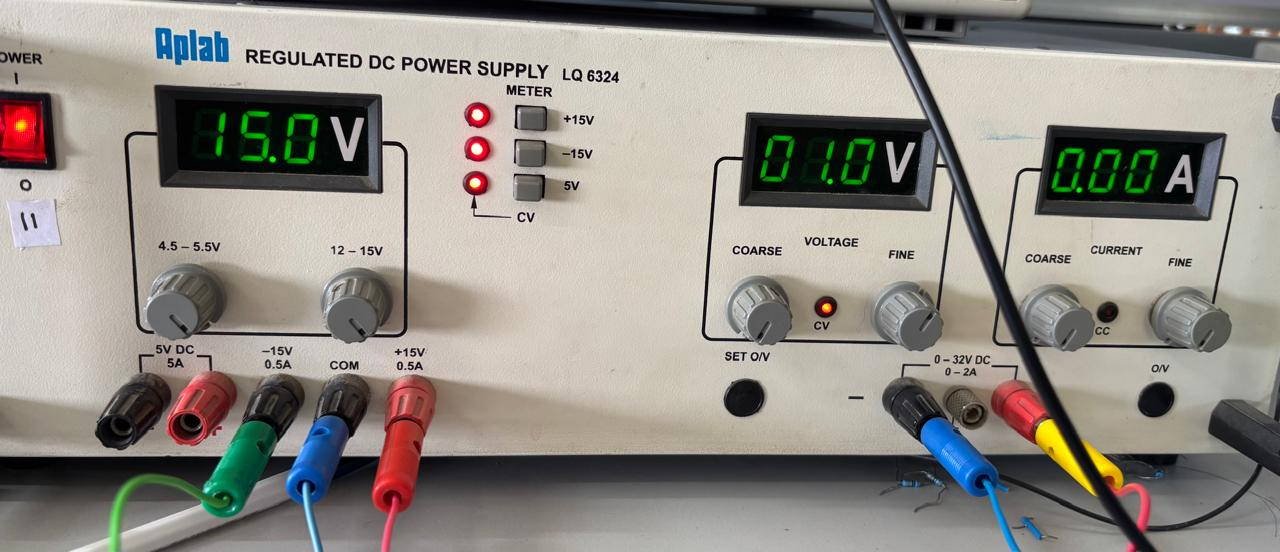
\includegraphics[width=\columnwidth]{figs/input1.png}
   \caption{Input}
\end{figure}
\pagebreak
\begin{figure}[!h]
	\begin{subfigure}[b]{100pt}
		\caption{Output}
		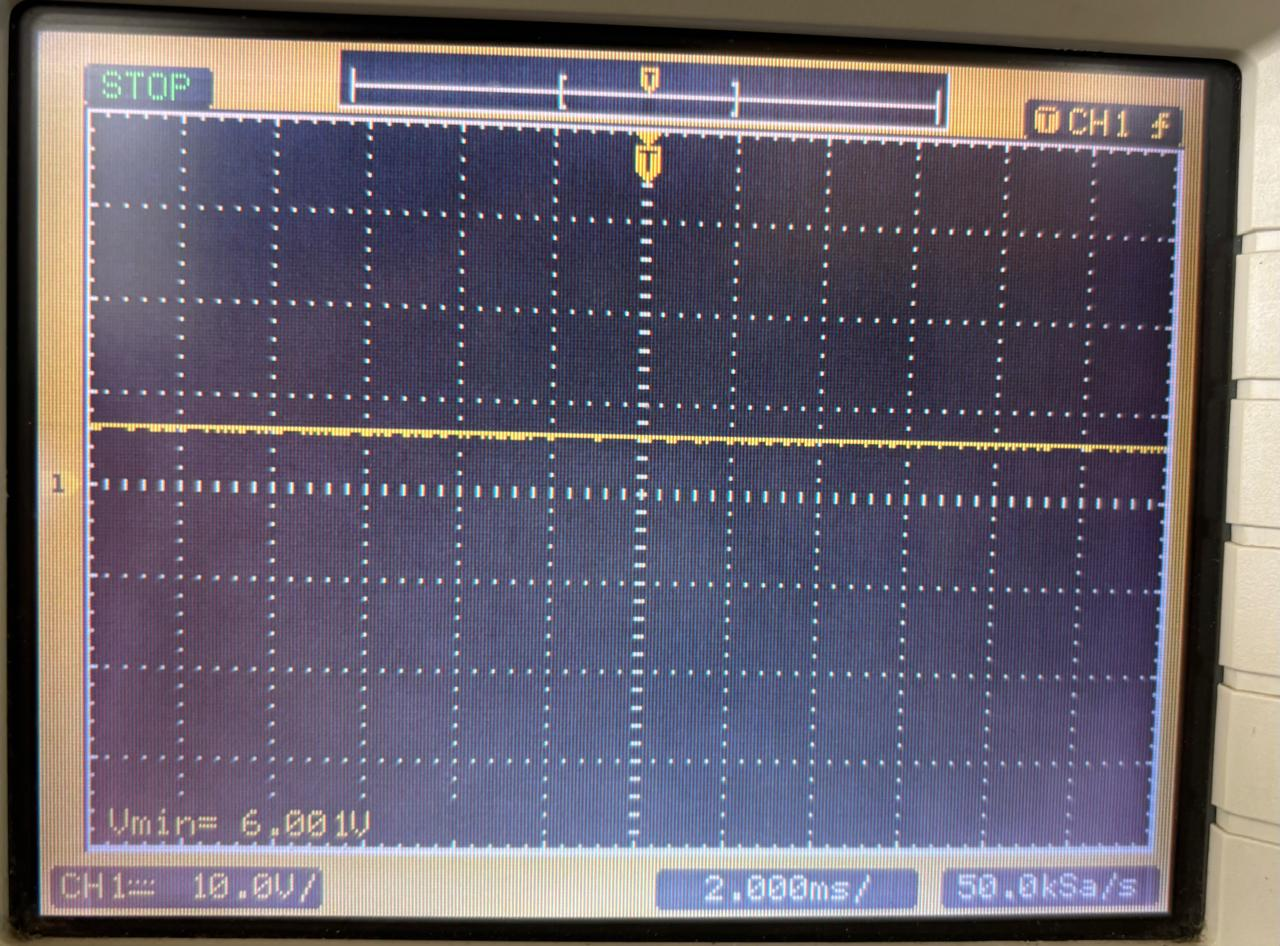
\includegraphics[width = 260pt]{figs/1add1.png}
	\end{subfigure}
	\hspace{110pt}
	\begin{subfigure}[b]{100pt}
		\caption{Circuit}
		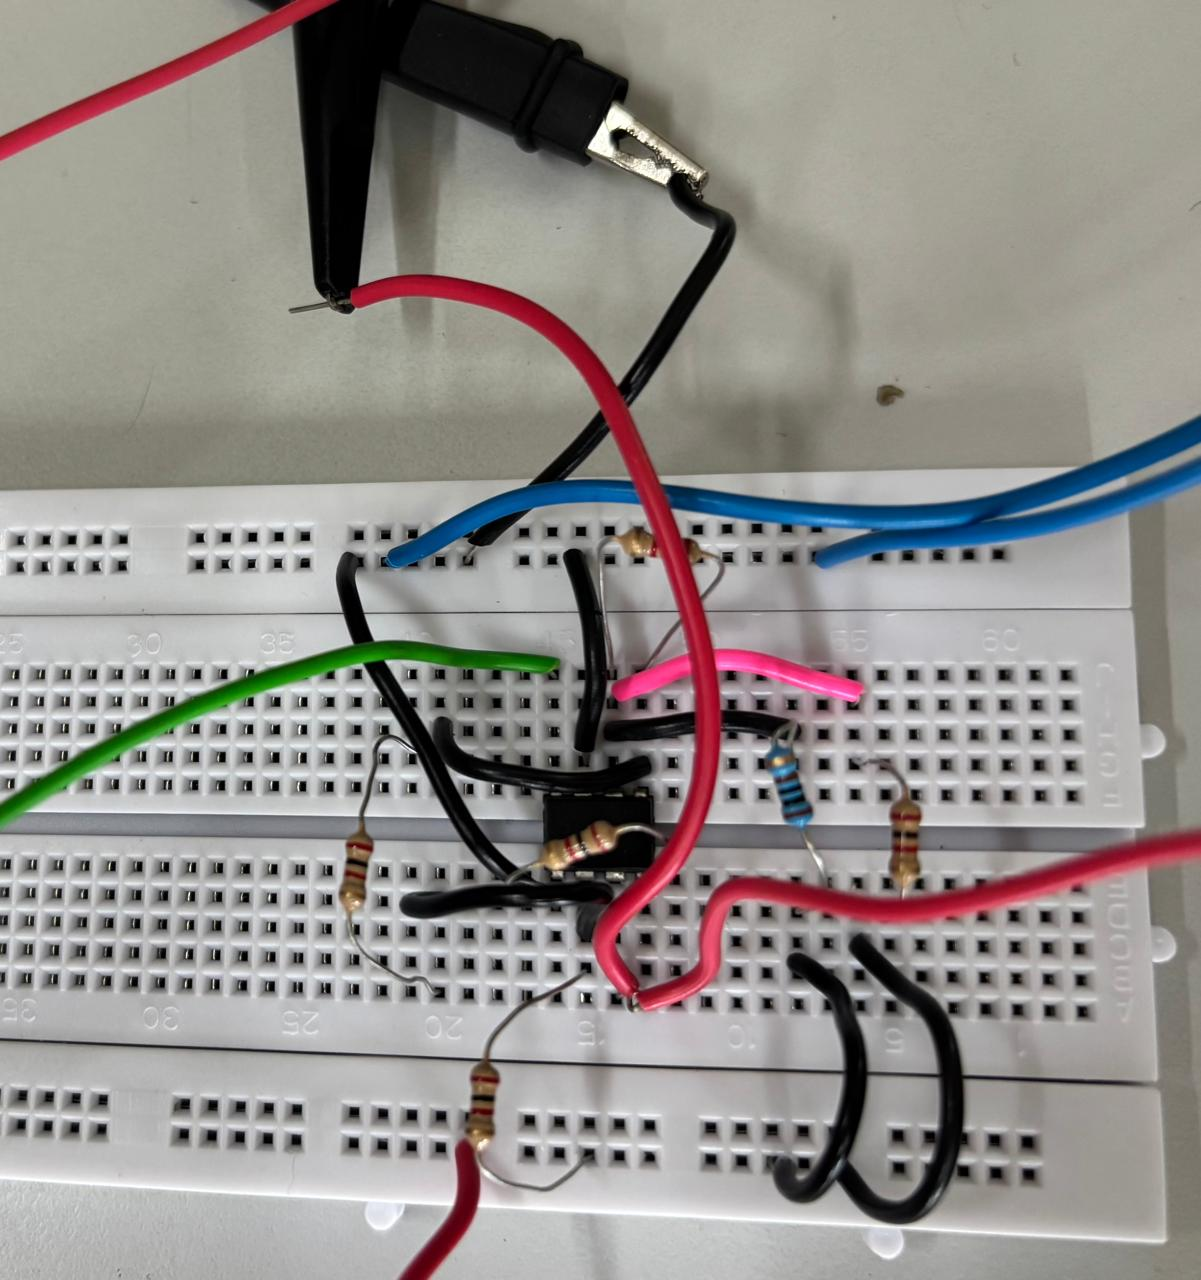
\includegraphics[width = 180pt]{figs/1add2.png}
	\end{subfigure}
\end{figure}
\pagebreak
\subsubsection*{$2V_1 - V_3$}
Here, $V_1 = 5V, V_3 = 1V$, \begin{align*}2V_1-V_3 = 6V\end{align*}
\begin{figure}[h!]
   \centering
   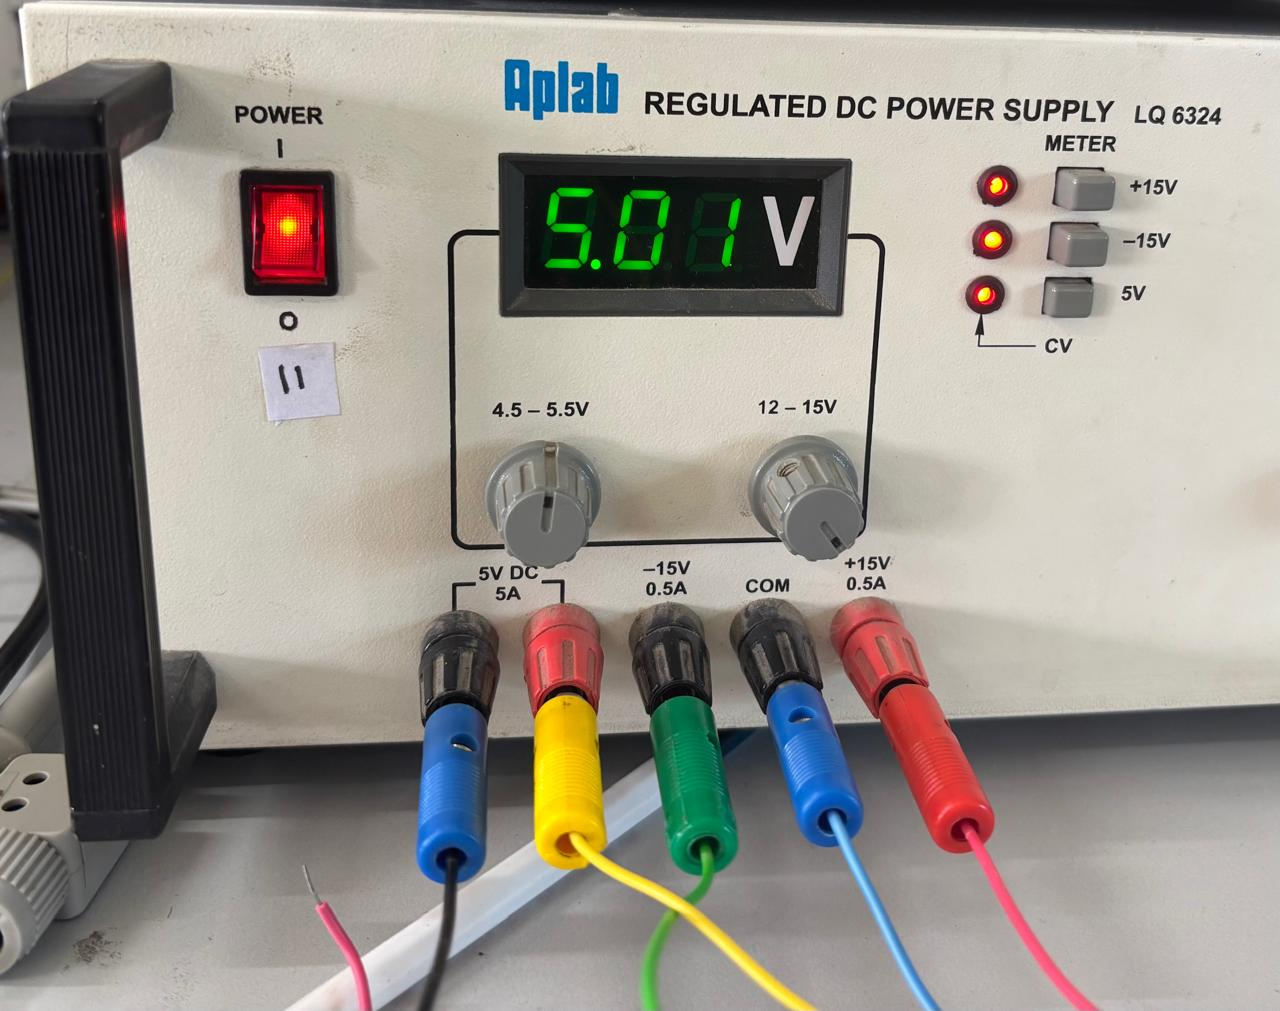
\includegraphics[scale = 0.2]{figs/input2.png}
   \caption{Input}
\end{figure}
\begin{figure}[!h]
	\begin{subfigure}[b]{100pt}
		\caption{Output}
		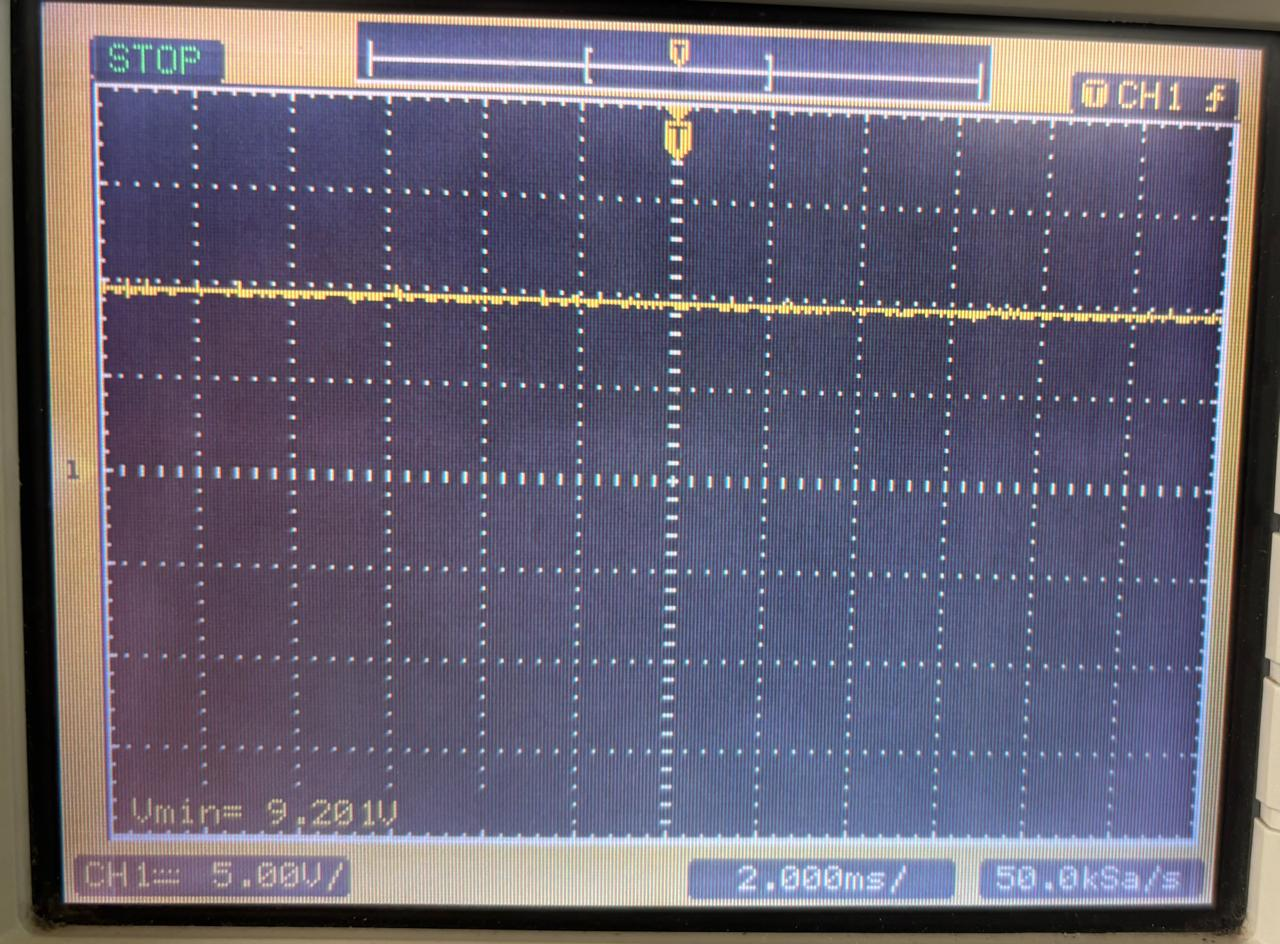
\includegraphics[width = 290pt]{figs/2add1.png}
	\end{subfigure}
	\hspace{110pt}
	\begin{subfigure}[b]{100pt}
		\caption{Circuit}
		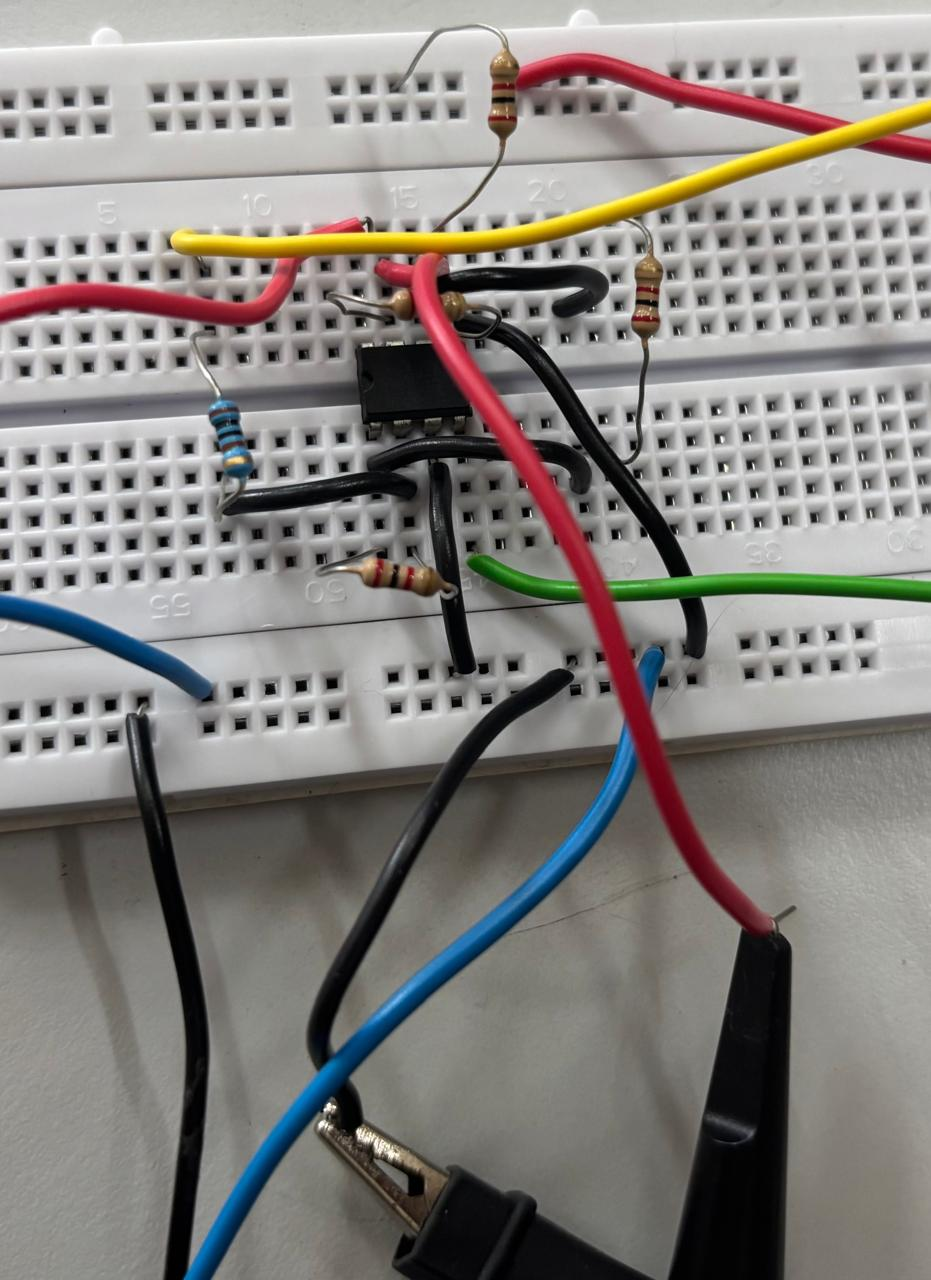
\includegraphics[width = 157pt]{figs/2add2.png}
	\end{subfigure}
\end{figure}

\pagebreak
\subsection*{Integrator Op-Amp}
Here, input wave is a square wave (triangle), so its integration will result in a triangle wave. Amplitude of triangle wave will be $\frac{t}{2RC}V_{max}$. \newline Here, $R = 10k\Omega, C = 10\mu F, V_{max} = 4V, t = 10 ms$. So, amplitude comes out to be $200mV$
\begin{figure}[!h]
	\begin{subfigure}[b]{100pt}
		\caption{Output vs Input}
		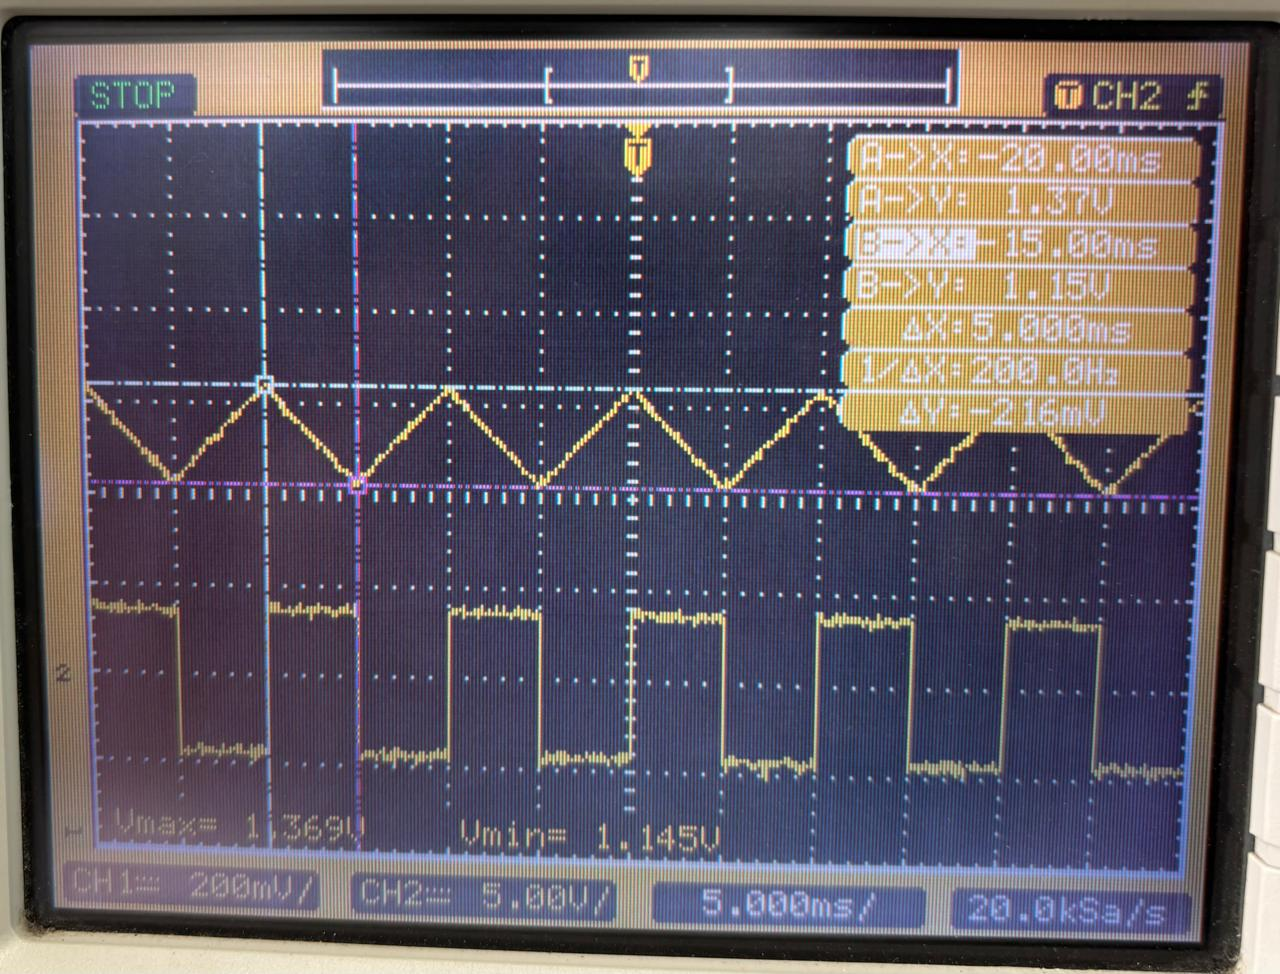
\includegraphics[width = 230pt]{figs/int1.png}
	\end{subfigure}
	\hspace{110pt}
	\begin{subfigure}[b]{100pt}
		\caption{Circuit}
		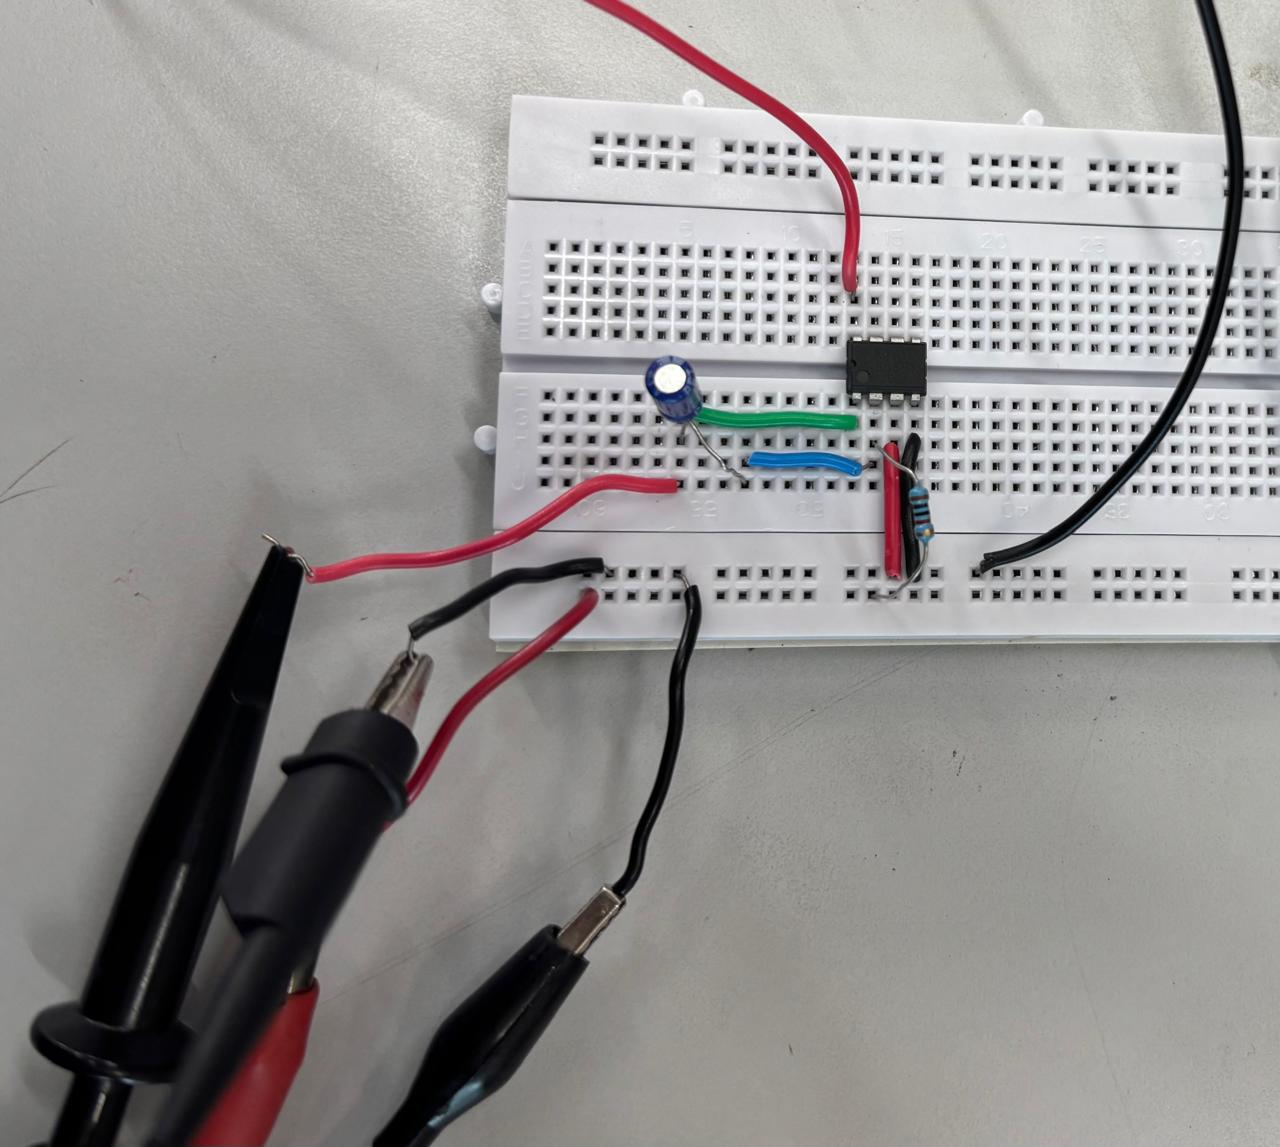
\includegraphics[width = 196pt]{figs/int2.png}
	\end{subfigure}
\end{figure}
\subsection*{Rectifier}
\subsubsection*{Half-Wave}
\begin{figure}[!h]
	\begin{subfigure}[b]{100pt}
		\caption{Output vs Input}
		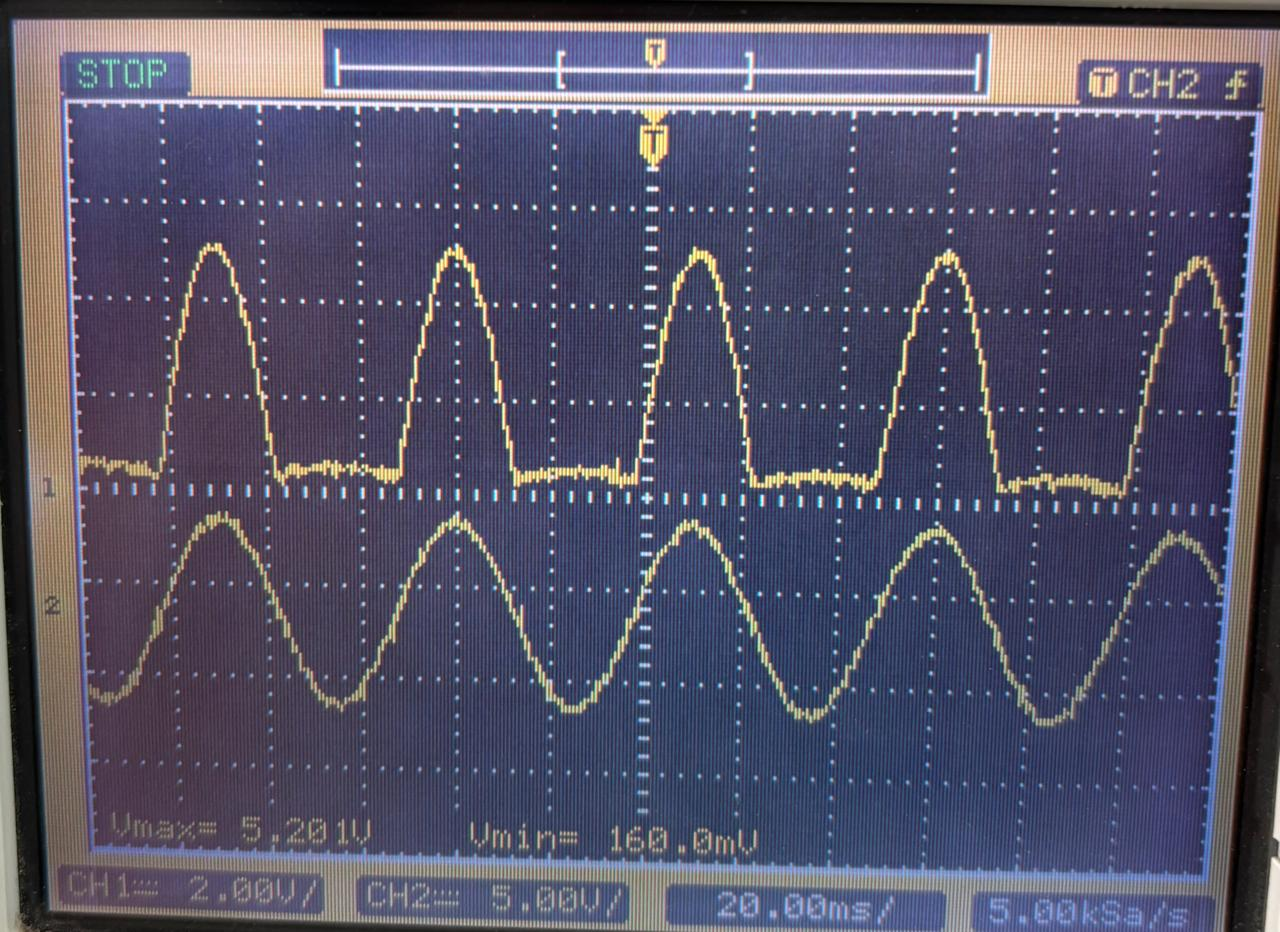
\includegraphics[width = 230pt]{figs/half1.png}
	\end{subfigure}
	\hspace{110pt}
	\begin{subfigure}[b]{100pt}
		\caption{Circuit}
		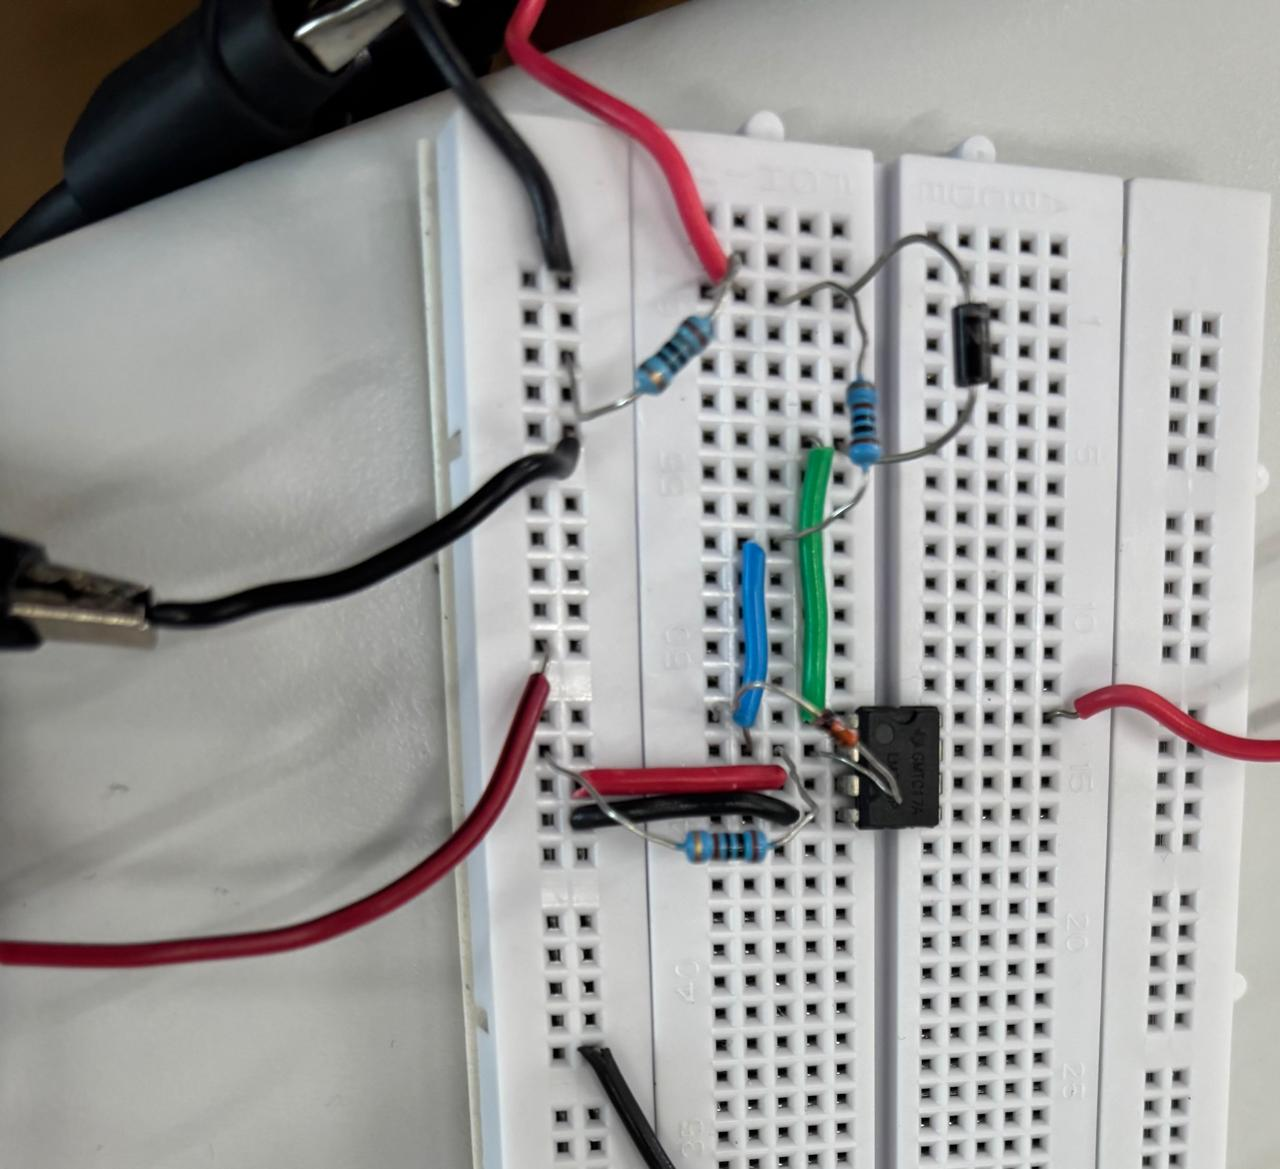
\includegraphics[width = 183pt]{figs/half2.png}
	\end{subfigure}
\end{figure}
\pagebreak
\subsubsection*{Full-Wave}
\begin{figure}[!h]
	\begin{subfigure}[b]{100pt}
		\caption{Output vs Input}
		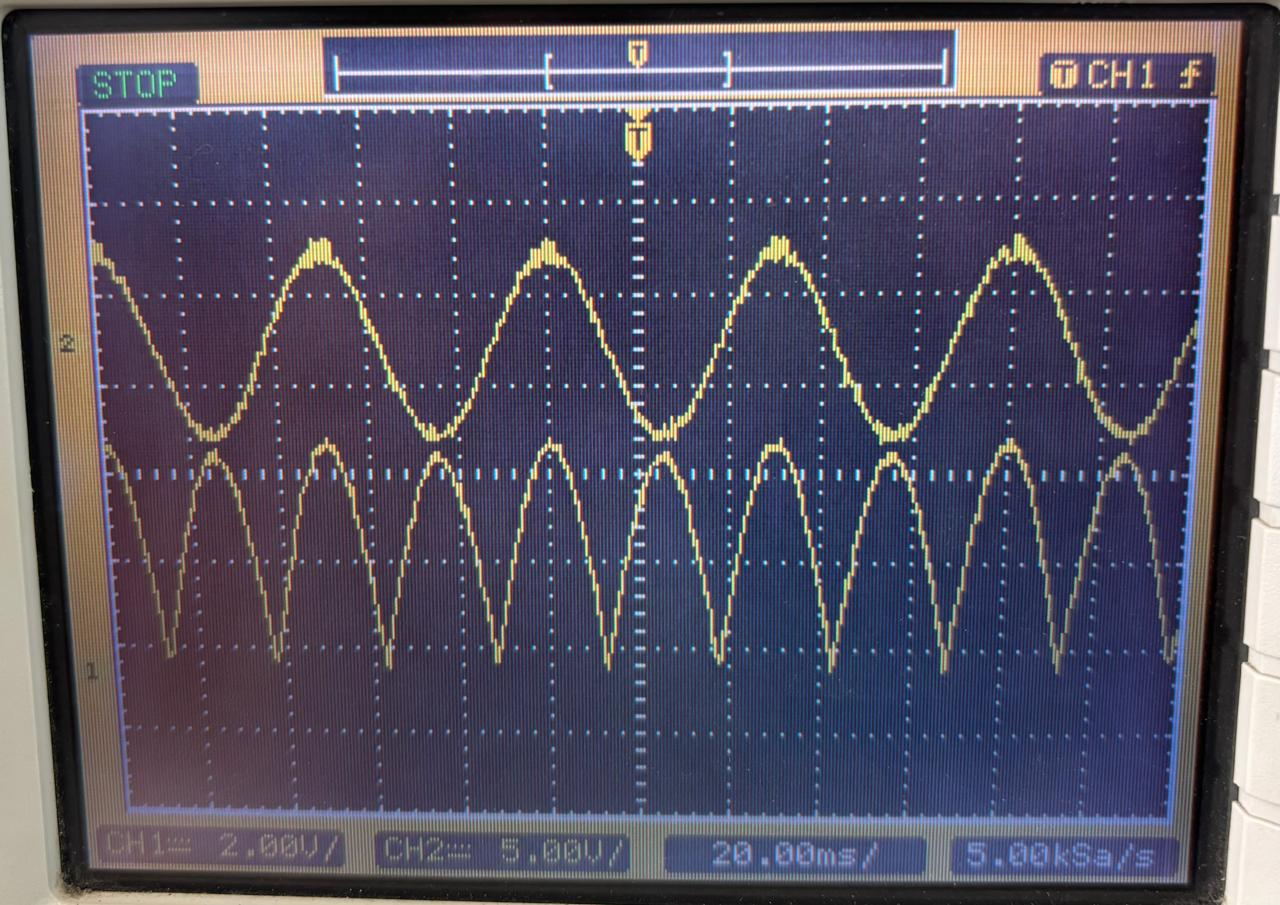
\includegraphics[width = 230pt]{figs/full1.png}
	\end{subfigure}
	\hspace{110pt}
	\begin{subfigure}[b]{100pt}
		\caption{Circuit}
		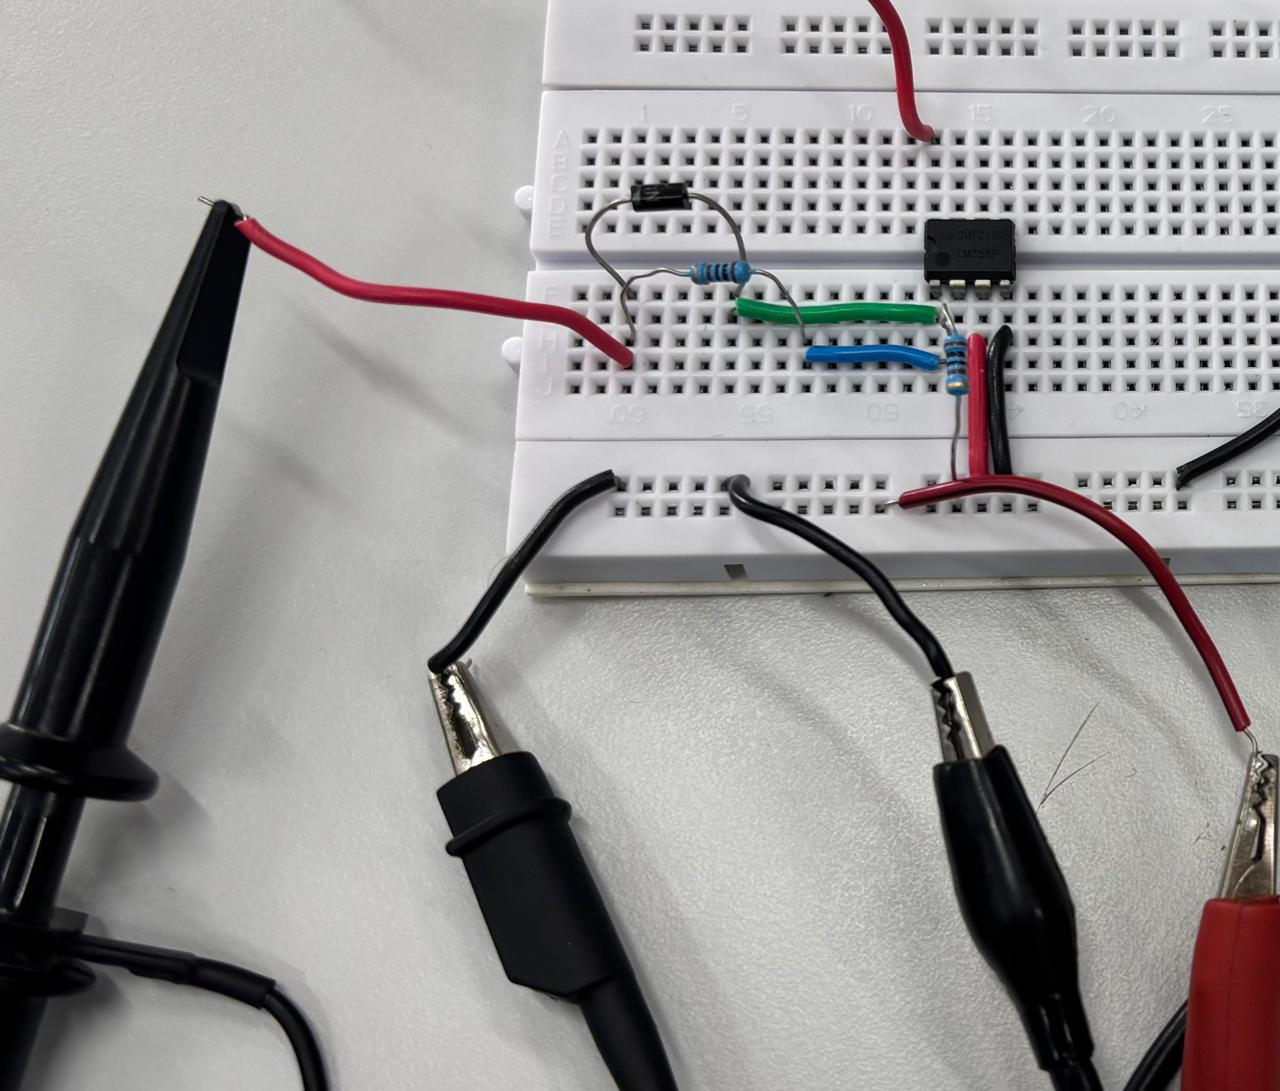
\includegraphics[width = 192pt]{figs/full2.png}
	\end{subfigure}
\end{figure}

\section*{Conclusion}
The experiment successfully demonstrated the functionality of different op-amp applications, including summing and difference amplification, integration, and precision rectification. The observed outputs were consistent with theoretical calculations, validating the practical applications of operational amplifiers.

\end{document}

